\chapter{Resultados \label{chap:Resultados}}
%%%%%%%%%%%%%%%%%%%%%%%%%%%%%%%%%%%%%%%%%%%%%%%%%%%%%%%%%%%%%%%%%%
%%%%%%%%%%%%%%%%%%%%%%%%%%%%%%%%%%%%%%%%%%%%%%%%%%%%%%%%%%%%%%%%%%
\section{Ajuste de espectros}
\noindent Habiendo calculado los valores de expectación de eventos de un electrón genuinos, es decir, difundidos desde un cluster de interés, $\mu_{g}$; y eventos de un electrón de fondo sobre un cluster o en su frontera, $\mu_{bkg}$, para corregir la carga sobre los clusters, y habiendo introducido el modelo de la colección parcial de carga, están dadas las condiciones para determinar las cantidades de interés: factor de Fano, energía de creación electrón hueco y ancho efectivo de la zona de colección parcial de carga.

Los resultados que se presentan a continuación son tanto para el pico generado por los rayos $X$ emitidos por el flúor como para el pico de los rayos $X$ emitidos por el aluminio. Para ambos casos se muestran los histogramas de carga con sus respectivos ajustes, utilizando el modelo descripto en la Capítulo \ref{chap:ModeloPCC}, para el caso en el que se aplicó el umbral \verb|EPIX=1.5| con las correcciones al sesgo introducido derivadas en el Capítulo \ref{chap:Analisis}. 
Se presentan los resultados tanto para el primer cuadrante del sensor como para el tercer cuadrante, debido a que el segundo cuadrante no funciona correctamente y el cuarto cuadrante presenta muchas \textit{hot columns}.

%%%%%%%%%%%%%%%%%%%%%%%%%%%%%%%%%%%%%%%%%%%%%%%%%%%%%%%%%%%%%%%%%%
%%%%%%%%%%%%%%%%%%%%%%%%%%%%%%%%%%%%%%%%%%%%%%%%%%%%%%%%%%%%%%%%%%
\subsection{Aluminio}
\noindent Utilizando el modelo descripto en el Capítulo \ref{chap:ModeloPCC}, se aplicó el método de la máxima verosimilitud para determinar los estimadores de $\mu$, $\sigma$ y $\beta$. Esto se logro realizando un barrido en el parámetro $\beta$, optimizando $\mu$ y $\sigma$ en cada paso. Asi se obtuvieron las curvas de la Figura \ref{fig:Al_barridos_beta}. En ellas se presenta el logaritmo de la verosimilitud para los cuadrantes uno y tres del sensor en función del parámetro $\beta$. De estas curvas se obtiene $\hat{\beta}$, que el valor de $\beta$ que maximiza la verosimilitud, y con él, queda determinado el conjunto de parámetros óptimos ($\hat{\mu}$, $\hat{\sigma}$, $\hat{\beta}$). A partir de $\hat{\mu}$, $\hat{\sigma}$ y su errores, se determinan los valores de $F$, $\varepsilon_{\eh}$ y sus errores por propagación. En los gráficos de la Figura \ref{fig:Al_barridos_beta} se muestra además la recta que se encuentra a una distancia $a=1/2$ por debajo del máximo y su intersección con la curva, de donde se obtuvieron los intervalos $[0.004; 0.011]$ y $[0.014; 0.023]$ para un $68.3\,\%$ de probabilidad de contener a $\beta$, para el primer y tercer cuadrante del sensor respectivamente. 

El tamaño de la región de PCC, junto con su error se desprenden de los valores hallados para $\beta$ y de la distancia de atenuación para los rayos $X$ del aluminio de $1486\,\si{eV}$, que en este caso vale $\tau_{\scaleto{X}{4pt}} = 8.087\,\si{\mu m}$\cite{AttenuationLength}. Utilizando que $\tau_{\scaleto{CCE}{4pt}} = \beta \tau_{\scaleto{X}{4pt}}$ se obtiene que $\tau_{\scaleto{CCE}{4pt}} = algo \pm otra cosa$.
\begin{figure}[h]
    \centering
        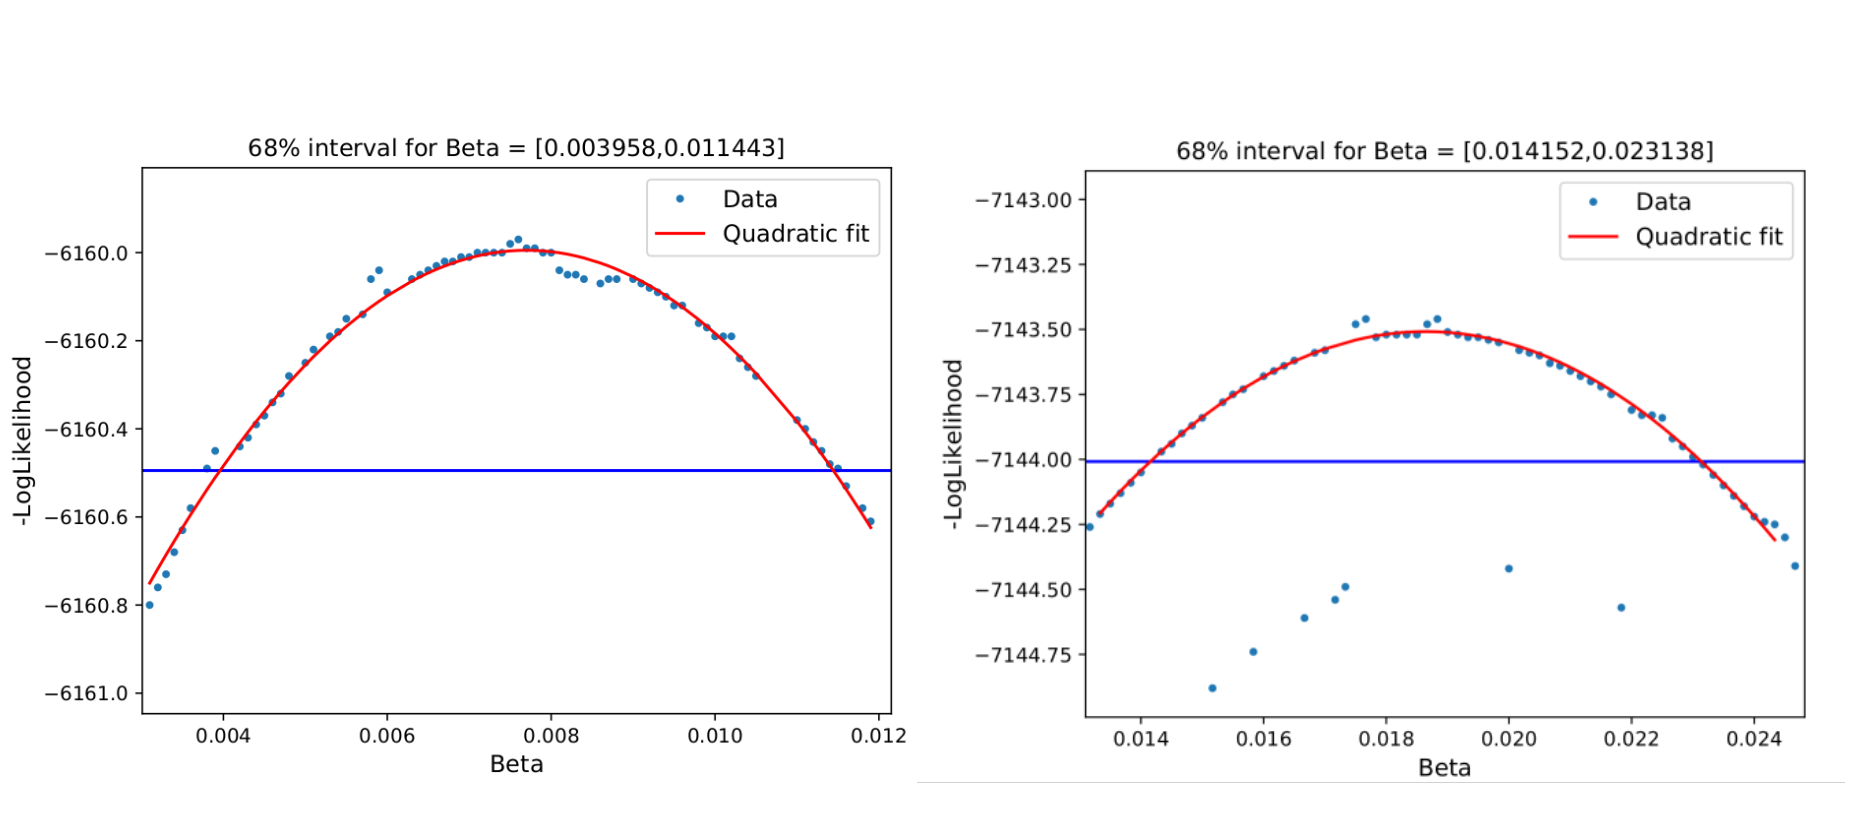
\includegraphics[scale=0.25]{pngs/Al_barridos_beta.png}
    \caption{Curvas del logaritmo de la verosimilitud en función de $\beta$, para los cuadrantes uno y tres con rayos $X$ del aluminio. Del ajuste cuadrático se obtiene el $\hat{\beta}$ máximo y de su intersección con la recta a a altura $\ln{(L(\hat{\beta}))} - 1/2$, los extremos de los intervalos.}
    \label{fig:Al_barridos_beta}
\end{figure}
Los valores óptimos obtenidos de los ajustes se encuentran condensados en la Tabla \ref{tab:Al_FanoEehOHDU1y3}.
\begin{table}[h]
\centering
\begin{tabular*}{\textwidth}{c @{\extracolsep{\fill}} ccccc}
%\begin{tabular}{@{}ccccc@{}}
\toprule
                & \multicolumn{2}{c}{OHDU1}                 & \multicolumn{2}{c}{OHDU3}                 \\ \hline\hline
                & $F$                 & $\varepsilon_{\eh}$ & $F$                 & $\varepsilon_{\eh}$ \\
EPIX 0.5 & $0.1322 \pm 0.0022$ & $3.7141 \pm 0.0019$ & $0.1498 \pm 0.0101$ & $3.7209 \pm 0.0029$ \\ 
EPIX 1.5 & $0.1455 \pm 0.0098$ & $3.7379 \pm 0.0024$ & $0.1699 \pm 0.0150$ & $3.7419 \pm 0.0039$ \\ 
EPIX 1.5 Corr & $0.1464 \pm 0.0096$ & $3.7501 \pm 0.0006$ & $0.1504 \pm 0.0011$ & $3.7485 \pm 0.0039$ \\ \bottomrule \hline
\end{tabular*}
\caption{Magnitudes de interés obtenidas del ajuste de los histogramas de carga de los rayos $X$ del aluminio para cada uno de los pasos del análisis. El primer paso es con el umbral en $0.5$, el segundo paso es con el nuevo umbral en $1.5$ y el tercer paso es con el nuevo umbral y con las correcciones a la carga de los clusters.}
\label{tab:Al_FanoEehOHDU1y3}
\end{table}
De esta se puede ver que el valor del factor de Fano aumenta al pasar de \verb|EPIX=0.5| a \verb|EPIX=1.5|, al mismo tiempo que sus incertezas, tanto para el primer cuadrante como para el tercero, lo cual no era un resultado anticipable dado el aumento de estadística. El factor de Fano aumenta $\sim 10\,\%$ y su incerteza aumenta más de $4$ veces para el primer cuadrante, mientras que para el tercero el factor de Fano aumenta $\sim 12\,\%$y su incerteza un $\sim 50\,\%$.

Al aplicar las correcciones respecto al paso anterior lo que se obtiene es una ligera disminución del valor del Fano para el primer cuadrante, menor al $1\,\%$, y otra no tan ligera disminución para el tercero, cerca del $\sim 12\,\%$, donde curiosamente las incertezas no se comportan de la misma manera para ambos casos: para el primer cuadrante la incerteza aumenta levemente, $\sim 3\,\%$, mientras que para el tercero disminuye muchísimo, mas del $\sim 95\,\%$. Todo esto puede verse con mayor claridad en el gráfico inferior derecho de la Figura \ref{fig:Al_mu_sigma_fano_eh}. Cabe destacar que los valores del factor de Fano para ambos cuadrantes se solapan con su error, de forma que los resultados para ambos cuadrantes resultan compatibles.
\textcolor{red}{como resultado final final del fano tenes que hacer el promedio pesado de los dos cuadrantes, lo mismo con la energía de creación electrón hueco} 
En los gráficos de la Figura \ref{fig:Al_OHDU1y3_EPIX15_Corr} se pueden ver los histogramas de carga generadas por la interacción de los rayos $X$ emitidos por el aluminio con su ajuste, obtenidos de los datos procesados con el umbral y las correcciones aplicadas, para los cuadrantes uno y tres, fijando el valor de $\beta$ en el máximo obtenido anteriormente para derivar el $F$ y $\varepsilon_{\eh}$ óptimos. En cada gráfico se encuentran superpuestos dos histogramas de carga: el histograma de carga con umbral \verb|EPIX=1.5| y superpuesto encima de este, el histograma de carga con el umbral \verb|EPIX=1.5| más las correcciones, con el fin de poder identificar si existen diferencias apreciables entre ambos. De esta forma se observa que las correcciones no modifican cualitativamente los histogramas.
\begin{figure}[h]
    \centering
        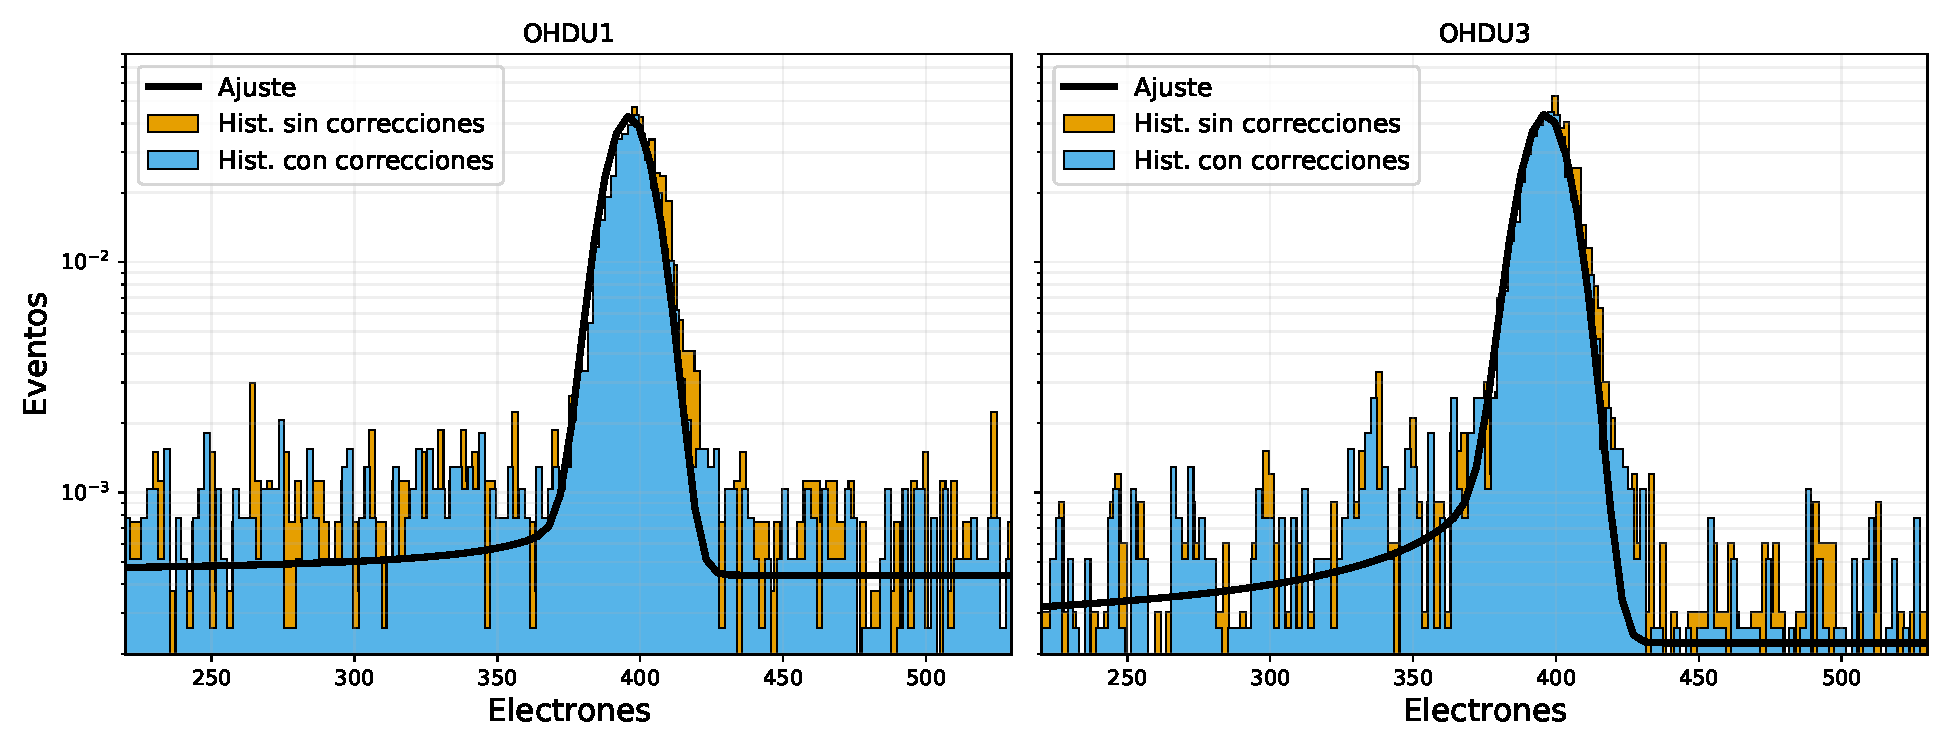
\includegraphics[scale=0.5]{Figs/Al_hists_ohdu1y3_dobles.pdf}
    \caption{Histogramas y ajustes del pico de los rayos $X$ del aluminio utilizando el modelo. El efecto de la colección parcial de carga es leve pero apreciable. Se superpusieron el histograma de carga con el nuevo umbral y el histograma de carga con el umbral más las correcciones en un mismo gráfico. No hay diferencias significativas en los histogramas.}
    \label{fig:Al_OHDU1y3_EPIX15_Corr}
\end{figure}
Observando el gráfico del factor de Fano y la dispersión de los picos en la Figura \ref{fig:Al_mu_sigma_fano_eh} se puede notar que el aumento en el valor de $F$ al aplicar el umbral se debe a un aumento de $\sigma$, %Es decir, al aumentar la estadística también aumenta el ancho de los picos \textcolor{red}{pareciera decirse que los picos se ensanchan porque hay mas estadística, y eso no tiene mucho sentido. Algo con el corte es el responsable, no me queda claro porqué, pero no lo diría de esta manera}
y la tendencia del factor de Fano es mayormente regida por esta.

En cuanto a la energía de creación electrón-hueco, para cada paso del análisis su valor aumentó, como puede verse en el gráfico inferior izquierdo de la Figura \ref{fig:Al_mu_sigma_fano_eh}. En este caso el aumento de la estadística y las correcciones implementadas compatibilizaron los resultados entre los dos cuadrantes dado que sus incertezas se solapan y sus valores absolutos difieren menos de $0.1\,\%$. Por su lado, la energía de creación electrón hueco acompaña claramente la tendencia contraria que sigue el valor medio de carga y esto se debe a que la forma en la que se la calcula es a partir de esta, como el cociente entre la energía inicial y el valor medio de carga, el cual está muy bien determinado.
\begin{figure}[h]
    \centering
        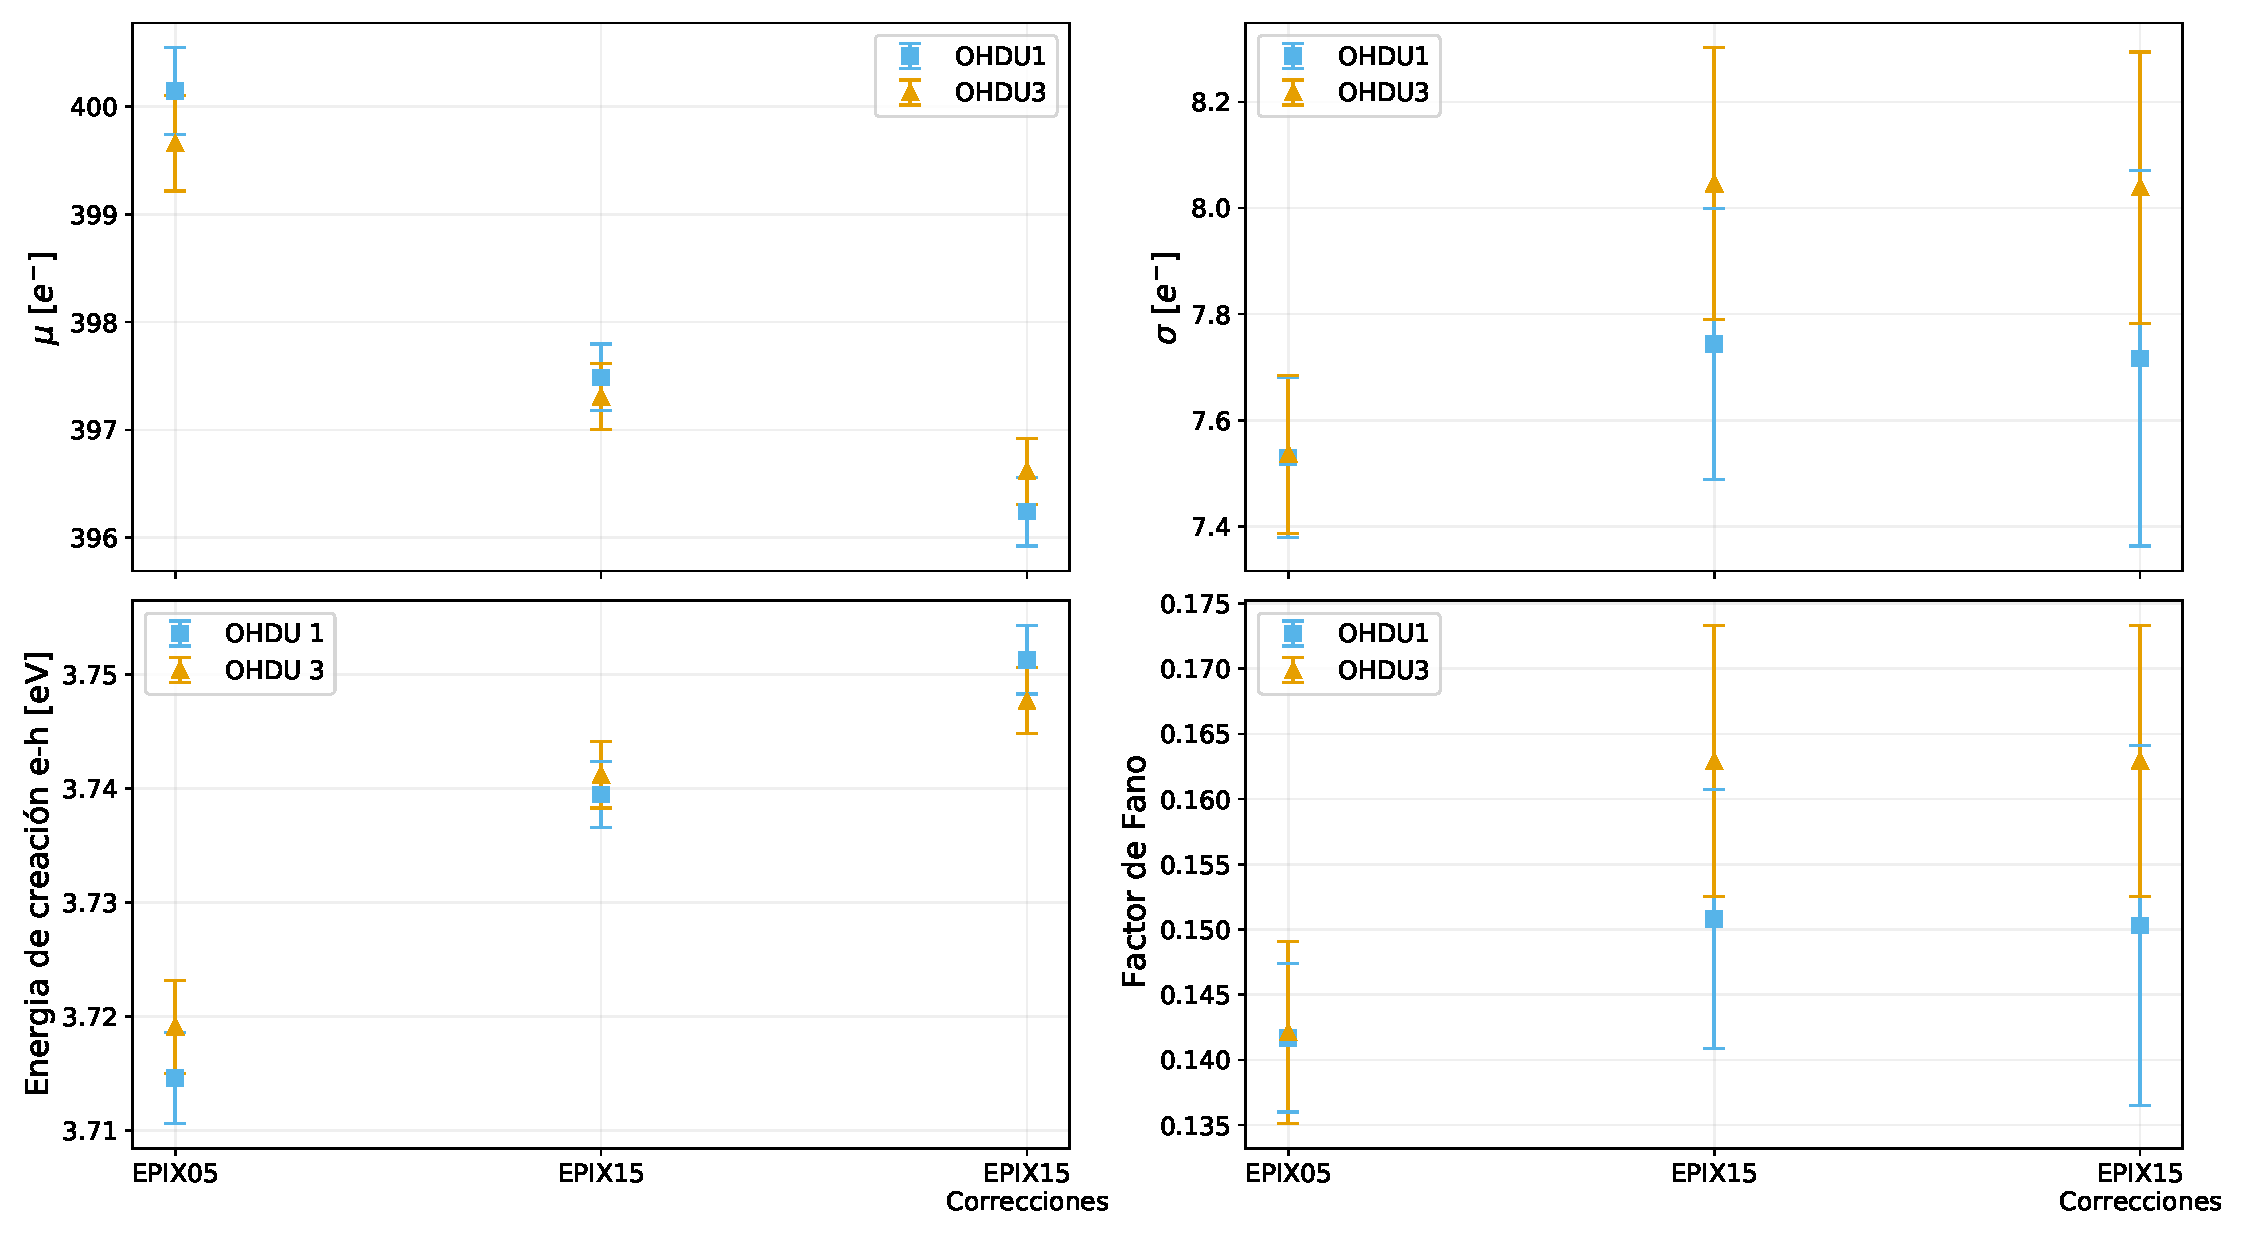
\includegraphics[scale=0.45]{Figs/Al_mu_sigma_fano_Eeh.pdf}
    \caption{Valores para las magnitudes relevantes para el factor de Fano y la energía de creación electrón hueco, cuadrantes uno y tres, para los tres pasos de análisis implementados. Izquierda-arriba: Valor medio del pico de rayos $X$ del aluminio; izquierda-abajo: Energía de creación electrón hueco; derecha-arriba: Dispersión de los picos; derecha-abajo: factor de Fano. Se observa que la tendencia del factor de Fano sigue la misma tendencia que la dispersión de los picos y que la energía de creación electrón-hueco la tendencia contraria al valor medio, lo cual es esperado porque se calcula a partir de esta.}
    \label{fig:Al_mu_sigma_fano_eh}
\end{figure}

%%%%%%%%%%%%%%%%%%%%%%%%%%%%%%%%%%%%%%%%%%%%%%%%%%%%%%%%%%%%%%%%%%
%%%%%%%%%%%%%%%%%%%%%%%%%%%%%%%%%%%%%%%%%%%%%%%%%%%%%%%%%%%%%%%%%%
\pagebreak
\subsection{Flúor}
\noindent Repitiendo el análisis llevado a cabo para el aluminio, se realizaron barridos en $\beta$ para obtener las curvas del logaritmo de la verosimilitud, de las cuales se obtienen el $\hat{\beta}$ máximo y los extremos de su intervalo de confianza en cada cuadrante, como se ve en la Figura \ref{fig:F_barridos_beta}. %
En este caso se ve que la curva obtenida para el tercer cuadrante no se aproxima por una cuadrática y no fue ajustada, con lo cual usar $\ln{(\Lagr(\hat{\beta}))} - 1/2$ para establecer el intervalo de $68.3\,\%$ no es correcto. %
Sin embargo para el primer cuadrante el ajuste cuadrático está en muy buen acuerdo con los valores obtenidos y de estos se desprende $\hat{\beta} = 0.232$, con su intervalo $[0.220; 0.245]$ de $68.3\,\%$.

En este caso, sabiendo que la longitud de atenuación en el silicio para los rayos $X$ del flúor de $677\,\si{eV}$ es de $\tau_{\scaleto{X}{4pt}} = 0.941\,\si{\mu m}$\cite{AttenuationLength}, se obtiene que el ancho de la región de PCC del detector es de $\tau_{\scaleto{CCE}{4pt}} = 0.218\,\si{\mu m}$, contenido en el intervalo $[0.206; 0.231]\,\si{\mu m}$.
\begin{figure}[h]
    \centering
    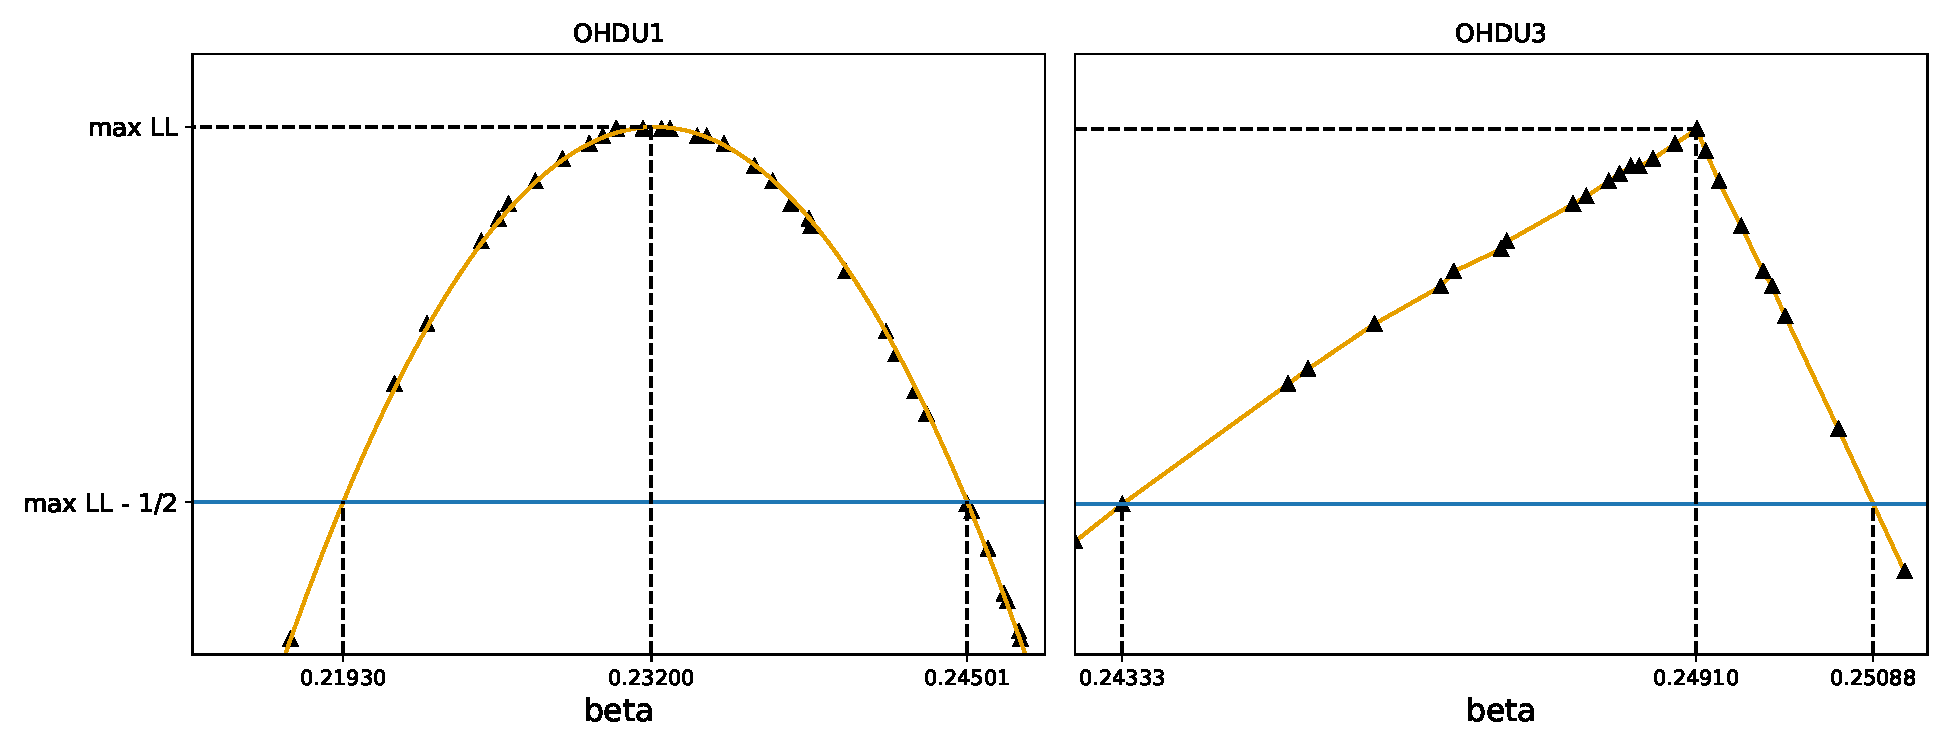
\includegraphics[scale=0.5]{Figs/F_barridos_beta.pdf}
    \caption{Curvas del logaritmo de la verosimilitud en función de $\beta$, para los cuadrantes uno y tres con rayos $X$ del flúor. Del ajuste cuadrático del primer cuadrante se obtiene el $\hat{\beta}$ máximo y de su intersección con la recta a a altura $\ln{(L(\hat{\beta}))} - 1/2$, los extremos de los intervalos. La curva para el tercer cuadrante no resultó ser cuadrática por lo cual no se realizó su ajuste, sin embargo se determina el intervalo dado por la intersección entre la recta a distancia $1/2$ de su máximo y la recta que une a los puntos que se encuentran de un lado y del otro de esta.}
    \label{fig:F_barridos_beta}
\end{figure}

Por otro lado, con el valor $\hat{\beta}$ hallado para el primer cuadrante, se realizaron los ajustes a los histogramas de carga de ambos cuadrantes y se obtuvieron los valores para el factor de Fano y energía de creación electrón-hueco. De la misma forma que para el aluminio, en la Figura \ref{fig:F_OHDU1y3_EPIX15conCorr} se tienen los histogramas de carga con y sin corrección, y con su respectivo ajuste. Se observa como la colección parcial de carga afecta a estos picos de forma mucho más importante que para el aluminio, formando colas muy pronunciadas a la izquierdo de estos. Esto es un resultado que se anticipaba en el Capítulo \ref{chap:ModeloPCC} y se debe al aumento del valor del parámetro $\beta$: como la longitud de atenuación para los rayos $X$ del flúor es mucho menor que la del aluminio, hay muchísimos más eventos que sufren recombinación en la región de PPC del sensor. En cuanto al ajuste, para este valor de $\beta$ se ve como la curva sigue muy bien las colas de los histogramas, tanto del lado izquierdo donde hay muchos eventos, como del lado derecho donde hay muchos menos. En la Tabla \ref{tab:F_FanoEehOHDU1y3} se presentan los resultados para los tres pasos del análisis para los cuadrantes uno y tres.
\begin{table}[h]
\centering
\begin{tabular*}{\textwidth}{c @{\extracolsep{\fill}} ccccc}
%\begin{tabular}{@{}ccccc@{}}
\toprule
                & \multicolumn{2}{c}{OHDU1}                 & \multicolumn{2}{c}{OHDU3}                 \\ \hline\hline
                & $F$                 & $\varepsilon_{\eh}$ & $F$                 & $\varepsilon_{\eh}$ \\
EPIX 0.5 & $0.1225 \pm 0.0112 $ & $3.6576 \pm 0.0006 $ & $0.1304 \pm 0.0106 $ & $3.6778 \pm 0.0050 $ \\ 
EPIX 1.5 & $0.1415 \pm 0.0202 $ & $3.7363 \pm 0.0097 $ & $0.1416 \pm 0.0120 $ & $3.7363 \pm 0.0065 $ \\ 
EPIX 1.5 Corr & $0.1415 \pm 0.0170 $ & $3.7363 \pm 0.0066 $ & $0.1417 \pm 0.0169 $ & $3.7363 \pm 0.0066$ \\ \bottomrule \hline
\end{tabular*}
\caption{Magnitudes de interés obtenidas del ajuste de los histogramas de carga de los rayos $X$ del aluminio para cada uno de los pasos del análisis. El primer paso es con el umbral en $0.5$, el segundo paso es con el nuevo umbral en $1.5$ y el tercer paso es con el nuevo umbral y con las correcciones a la carga de los clusters.}
\label{tab:F_FanoEehOHDU1y3}
\end{table}
En ambos cuadrantes se tiene que el factor de Fano aumenta junto con su incerteza al pasar de \verb|EPIX=0.5| a \verb|EPIX=1.5| y que al aplicar las correcciones, para el primer cuadrante el valor no se modifica pero su incerteza disminuye $\sim 15\,\%$ respecto de la anterior. En ambos casos la incerteza antes de aplicar el umbral y correcciones era menor, lo cual tampoco es un resultado anticipable. A pesar de que las barras de error compatibilizan ambos cuadrantes en los tres pasos del análisis, se observa que los valores absolutos se vuelven mucho más semejantes al aplicar umbral y correcciones, siendo $F=0.1415$ y $F=0.1417$ para los cuadrantes uno y tres respectivamente, mejorando aún más la compatibilidad entre ellos. Para la energía de creación electrón-hueco sucede lo mismo en ambos cuadrantes, pasar de \verb|EPIX=0.5| a \verb|EPIX=1.5| aumenta el valor de la magnitud y su incerteza, y al aplicar las correcciones hay una ligera disminución para el primer cuadrante. 
\begin{figure}[h]
    \centering
    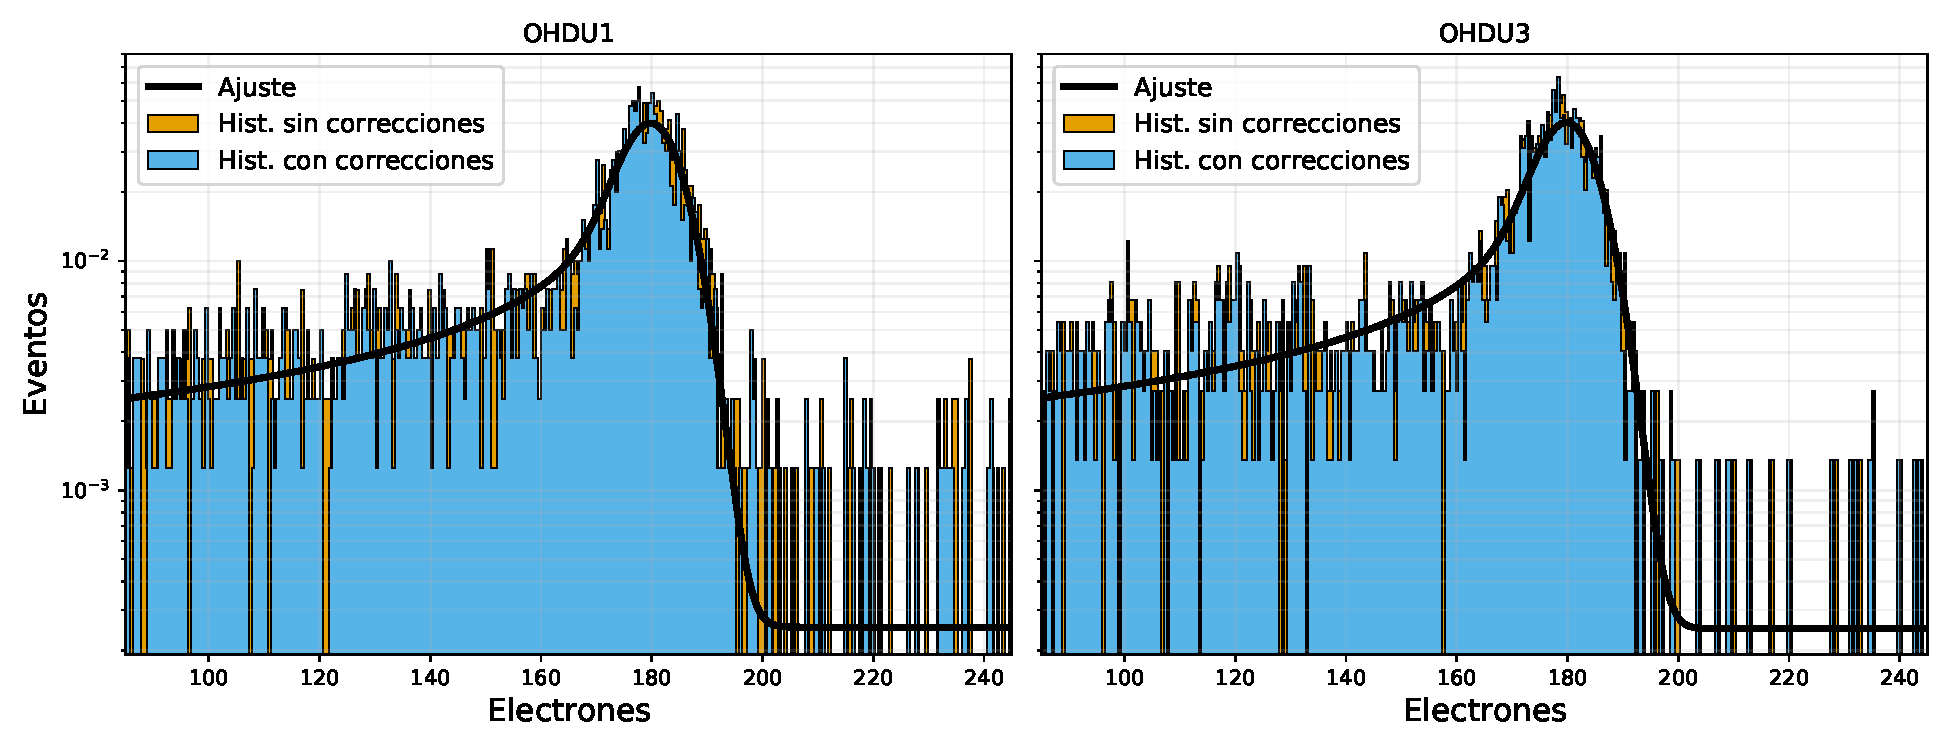
\includegraphics[scale=0.5]{Figs/F_hists_ohdu1y3_dobles.pdf}
    \caption{Histogramas y ajustes del pico de los rayos $X$ del flúor utilizando el modelo. El efecto de la colección parcial de carga es mucho más relevante en este caso, con gran cantidad de eventos a la izquierda del máximo del pico. Nuevamente se superponen el histograma de carga con el nuevo umbral y el histograma de carga con el umbral más las correcciones en un mismo gráfico. No hay se observan diferencias significativas ambos.}
    \label{fig:F_OHDU1y3_EPIX15conCorr}
\end{figure}
En los gráficos de la Figura \ref{fig:F_mu_sigma_fano_eh} se ven las tendencias de las magnitudes de interés con sus respectivos errores para cada uno de los análisis realizados. Para el caso del factor de Fano, se puede ver que sigue la misma tendencia que la dispersión, como sucedía para el aluminio y que los errores de ambos se solapan para los pasos. Sin embargo, al aumentar el umbral y aplicar las correcciones los valores absolutos se acercan mucho compatibilizándose aún más. La energía de creación electrón-hueco también se compatibiliza al aplicar el umbral y las correcciones.
\begin{figure}[h]
    \centering
        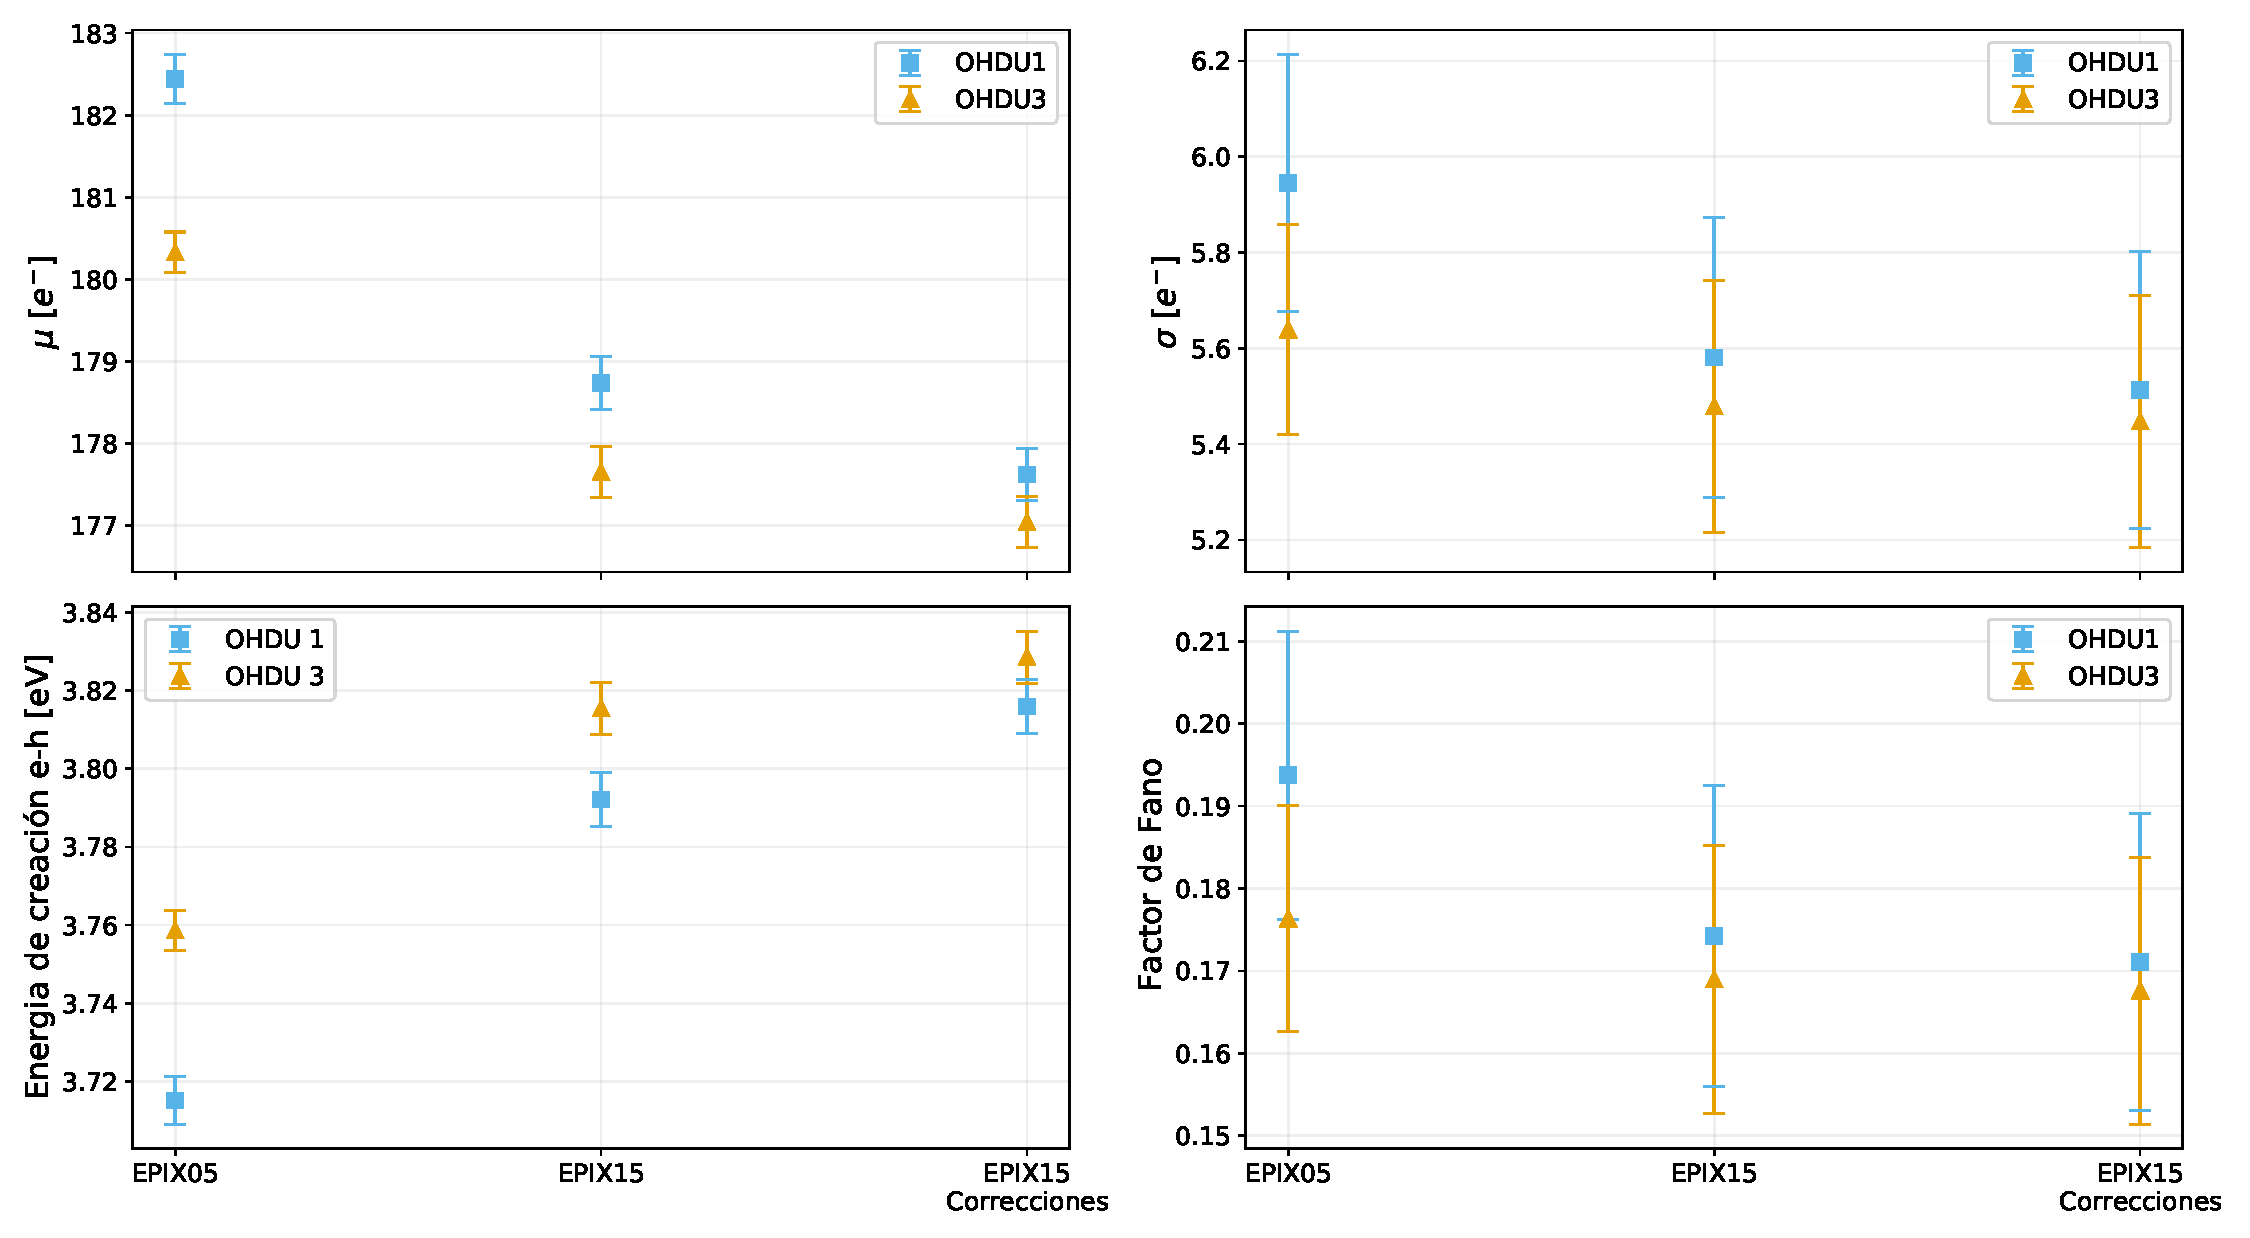
\includegraphics[scale=0.45]{Figs/F_mu_sigma_fano_Eeh.pdf}
    \caption{Valores para las magnitudes relevantes para el factor de Fano y la energía de creación electrón hueco, cuadrantes uno y tres, para los tres pasos de análisis implementados. Izquierda-arriba: Valor medio del pico de rayos $X$ del flúor; izquierda-abajo: Energía de creación electrón hueco; derecha-arriba: Dispersión de los picos; derecha-abajo: factor de Fano. Se observa que la tendencia del factor de Fano sigue la misma tendencia que la dispersión de los picos y que la energía de creación electrón-hueco la tendencia contraria al valor medio, lo cual es esperado porque se calcula a partir de esta.}
    \label{fig:F_mu_sigma_fano_eh}
\end{figure}

Finalmente, no se obtuvieron mejoras apreciables en las incertezas de las magnitudes a pesar del aumento de la estadística provocado por el nuevo umbral utilizado. Sin embargo, el procedimiento utilizado para la corrección de los sesgos logra compatibilizar los cuadrantes uno y tres tanto para el factor de Fano como para el energía de creación electrón-hueco, para los rayos $X$ del aluminio y del flúor. Por otro lado, estos resultados también ponen de manifiesto la ventaja de la utilización de este nuevo modelo de ajuste, debido a que a partir de este tipo de mediciones se puede obtener el ancho efectivo de la región de colección parcial de carga del detector.

Con estos resultados se puede actualizar el gráfico de la figura \ref{fig:Fano_y_ruido} y queda como se ven en la figura \ref{fig:Fano_y_ruido_final}, muy cercanos a la recta que representa el valor constante del factor de Fano en $F = 0.119$, correspondiente al valor obtenido para los rayos $X$ del $\Fe{55}$ en trabajos anteriores\cite{Rodrigues}.
\begin{figure}[H]
    \centering
        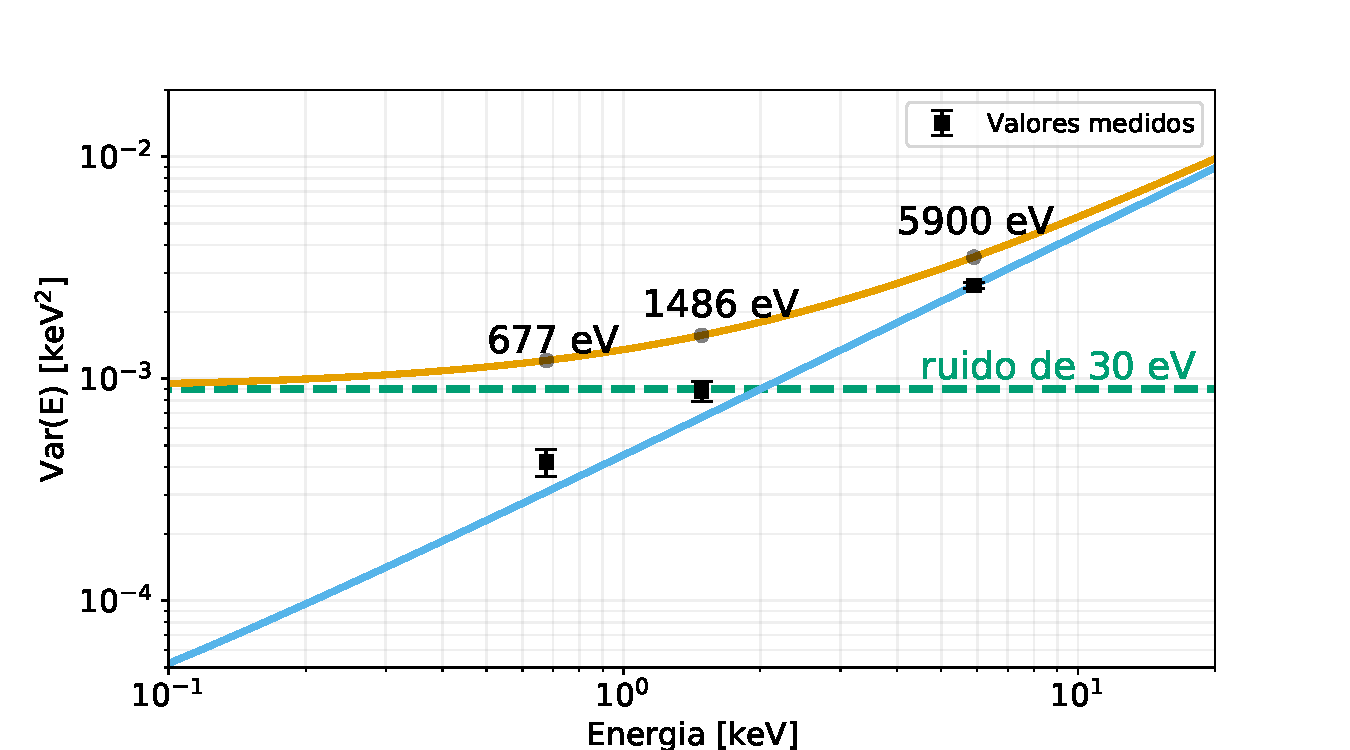
\includegraphics[scale=0.5]{Figs/FanoyRuidoFinal.pdf}
    \caption{Gráfico del factor de Fano obtenido de las mediciones y análisis realizados en este trabajo (cuadrados negros) comparado con la recta esperada si el factor de Fano fuera constante. También se grafica la curva y los valores con lo que mediría un CCD convencional para estas energias (puntos negros).}
    \label{fig:Fano_y_ruido_final}
\end{figure}